\documentclass[titlepage]{article}
\title{The watcher theme developing manual}
\author{Hiroaki Yamamoto}

\usepackage[dvipdfmx]{graphicx}
\usepackage[dvipdfmx]{hyperref}

\begin{document}
    \maketitle
    \tableofcontents
    \clearpage
    \section{What This Document?}
        This document describes how to create the theme files for watcher.
        
    \section{Identifier}
        All contents of each plugin have identifiers that is UUID. The identifier in the content may be changed when software execution, reloading, 
        and some situations modifying the contents is required. However, the identifier has very important feature.
        The identifier is used for resolving confliction between the contents: if 2 contents have the same names and different identifiers,
        the contents will be resolved properly because the identifiers are different. Additionally, if 2 contents have the same identifiers
        and different names, the contents will be resolved properly because the names are different
        (However, the confliction between the identifiers is very rare: The possiblity of the confliction is $\frac{1}{2^{61}}$, so almost zero).
        
        The UUID is passed as a string, so generated tab\ref{Tab} and buttons of contents must hold the string (i.e. UUID) as property named \verb@uuid@.
        Look at RootTabContent.qml and ButtonListView.qml in default theme for example.
        
    \section{File Formats and Required Files}
        The theme files are written QML and JSON. QML is used for the themes themselves, JSON is for versioning.
        At least, The files listed on Table\ref{required_files} are needed for the theme:
        
        \begin{table}[htb]
        \caption{Required files for the theme \label{required_files}}
            \begin{center}
                \begin{tabular}{|l|p{8cm}|}
                    \hline File Name&Description\\
                    \hline \verb@RootWindow.qml@&This file shows categories and boards per plugin.\newline
                                            Additionally,  This file is loaded and shown before other files are loaded. \\
                    \hline \verb@VersionWindow.qml@&This file shows the version of software and GPL.
                                    (In fact, this software doesn't have the version; GIT commit hash is used instead.)\\
                    \hline \verb@info.json@&Version Information File (\ref{versioning}) \\
                    \hline
                \end{tabular}
            \end{center}
        \end{table}
        
        For details, look at each section.

    \section{RootWindow.qml\label{RootWindow}}
        This file is loaded and shown before other files, and it has a feature to show Categories and Boards per plugin.
        The point is adjusting your theme to mine is unneeded; Creating a substitution for Tab(\ref{Tab}), 
        TabContents(\ref{TabContents}), creating signal on root object of this module(\label{required_signals_for_RootWindow}), 
        and the functions listed on Table.\ref{required_functions_for_RootWindow} that have described behaviors is only needed. 
        This means, you can create the design of Category Panel UI instead of Tab(\ref{Tab}) and TabContents(\ref{TabContents}) 
        as long as you are observing the rule of Tab System (\ref{Tab}) and TabContents System (\ref{TabContents}).
        
        \begin{table}[htb]
        \caption{Required signals for RootWindow.qml\label{required_signals_for_RootWindow}}
            \begin{center}
                \begin{tabular}{|l|p{8cm}|}
                    \hline Signal Name&Behavior \\
                    \hline \verb@currentTabChanged(var previous,var current)@&
                                This signal should be emitted when current selection of Tab(\ref{Tab}) is changed.
                                \verb@provious@ parameter should be an object selected previously, and 
                                \verb@current@ parameter should be an object selected currently.
                                These parameter is required, but they are not used on implementation; They may be used in the future.\\
                    \hline
                \end{tabular}
            \end{center}
        \end{table}
        
        \begin{table}[htb]
        \caption{Required functions for RootWindow.qml\label{required_functions_for_RootWindow}}
            \begin{center}
                \begin{tabular}{|l|p{8cm}|}
                    \hline Function Name&Behavior \\
                    \hline \verb@addTab(contentTitle,uuid)@&Create a TabContents(\ref{TabContents}) that has \verb@contentTitle@ as \verb@title@
                                                        and returns the created TabContents(\ref{TabContents}).
                                                        \verb@uuid@ is an identifier to resolve confliction.
                                                        The generated tab must hold \verb@uuid@ as the string property named "uuid"\\
                    \hline
                \end{tabular}
            \end{center}
        \end{table}
        
        In addition to these features, RootWindow.qml has "feature buttons" such as Bookmark Manager Button, Version Window Button,
        etc... And, at least, implementing the buttons listed on Table.\ref{required_buttons_for_RootWindow} are required.
        
        \begin{table}[htb]
        \caption{Required Buttons for RootWindow.qml\label{required_buttons_for_RootWindow}}
            \begin{center}
                \begin{tabular}{|l|p{8cm}|}
                    \hline Object Name      &Behavior \\
                    \hline \verb@back@      &Goes back. \\
                    \hline \verb@next@      &Goes next. \\
                    \hline \verb@reload@    &Reloads View. \\
                    \hline \verb@bookmark@  &Opens Bookmark Manager. \\
                    \hline \verb@config@    &Opens Configuration Window. \\
                    \hline \verb@save@      &Stores configuration as a file. \\
                    \hline \verb@open@      &Imports configuration from a file by using "save."\\
                    \hline \verb@info@      &Opens Version Window. \\
                    \hline \verb@exit@      &Exit watcher. \\
                    \hline
                \end{tabular}
            \end{center}
        \end{table}
        
        Note that implementing their behavior is unneeded;You only need to assign the Object Name described above to objectNmae property 
        of the corresponding button.
        
        For example, the default theme is designed like Figure.\ref{RootWindow_fig}.
        
            \begin{figure}[htb]
                \begin{center}
                    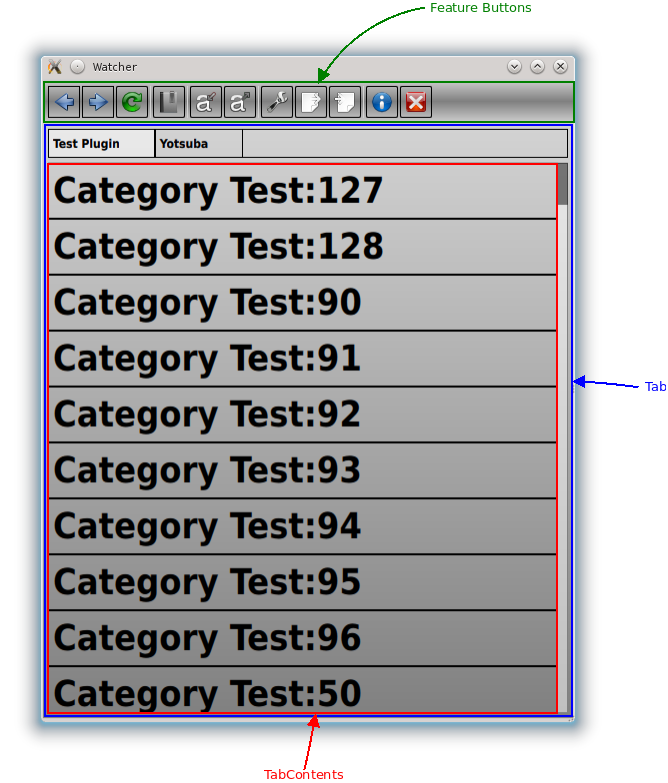
\includegraphics[scale=0.6]{img/RootWindow_structure.png}
                \end{center}
                \caption{The structure of RootWindow \label{RootWindow_fig}}
            \end{figure}
        
    \section{VersionWindow.qml}
        VersionWindow.qml is used for displaying the version of this software. In fact, this software doesn't have its version, 
        but using/displaying version has many profits. For example, showing copyright on VersionWindow is a very traditional idea.
        Additionally, this software uses GIT commit hash as a version, so bugs can be detected more efficiently than versioning.
        
        VersionWindow.qml has a simpler structure than RootWindow.qml. It has title area, copyright area, and close button.
        Note that copyright area may be very long. Therefore, designing a scrollable area will be required.
        
        The Context Properties listed on Table.\ref{additional_property_for_VersionWindow} are additional and usable properties on VersionWindow.
        
        \begin{table}[htb]
            \caption{Additional Properties on VersionWindow \label{additional_property_for_VersionWindow}}
            \begin{center}
                \begin{tabular}{|l|l|p{8cm}|}
                    \hline Name&Type&Description \\
                    \hline \verb@copyright@         &\verb@string@&String of Copyright \\
                    \hline \verb@applicationName@   &\verb@string@&the name of this software. i.e. "watcher". \\
                    \hline
                \end{tabular}
            \end{center}
        \end{table}
        
    \section{Tab System \label{Tab}}
    Tab system has listing plugin name, and TabContents (\ref {TabContents}). Clicking the list, the Tab switches to the corresponding TabContents, and
    displaying the content is changed. This interface has no required properties/methods, and you can design the futuristic tab like StackWidget, 
    Left Placed Column Tab, etc... However, when addTab on RootWindow.qml(\ref{RootWindow}) is invoked, the created TabContents should be added to this widget.
    
    \section{TabContents System \label{TabContents}}
    TabContents system is used for displaying Categories and boards.
    
    The system has title area and displaying area. Both of them are managed by roottabcontents.cxx. Therefore, required properties, signals,
    and functions exist. The required properties are listed on Table.\ref{required_properties_tabcontents}, signals are listed on 
    Table.\ref{required_signals_tabcontents}, functions are listed on \ref{required_functions_tabcontents}.
    
    \begin{table}[htb]
        \caption{Required Properties for TabContents System \label{required_properties_tabcontents}}
        \begin{center} \begin{tabular}{|l|l|p{4cm}|}
            \hline Property Name&Type&Description\\
            \hline \verb@title@             &\verb@string@                  &The title of plugin.\\
            \hline \verb@buttonClickedEvent@&\verb@lambda(sender_button)@   &When the element on TabContents is 
                                                                             clicked, this function is invoked.
                                                                             \verb@sender_button@ must be the object clicked by user.\\
            \hline \verb@hasAnimation@      &\verb@bool@                    &Specifys if the theme has a animation.
                                                                             If true, TabContents.cxx will call hide()
                                                                             before reading categories/boards list, and calls
                                                                             show() after reading categories/boards list.
                                                                             Otherwise the functions are not invoked.\\
            \hline
        \end{tabular} \end{center}
    \end{table}
    
    \begin{table}[htb]
        \caption{Required Signals for TabContents System \label{required_signals_tabcontents}}
        \begin{center} \begin{tabular}{|l|p{7cm}|}
            \hline Signal Name&Description \\
            \hline \verb@buttonClicked(sender_button)@  &When the element on TabContents is clicked, this signal is emitted.
                                                            \verb@sender_button@ must be the object clicked by user.\\
            \hline \verb@hideAnimationCompleted()@      &This signal should be emitted when hiding animation is completed.\\
            \hline \verb@showAnimationCompleted()@      &This signal should be emitted when {\bf showing} animation is completed.\\
            \hline
        \end{tabular} \end{center}
    \end{table}
    
    Note that {\bf \verb@sender_button@ on \verb@buttonClicked@ and \verb@buttonClickedEvent@ needs \verb@text@ property.}
    If the property doesn't exist, fetching categories/boards will fail.
    
    \begin{table}[htb]
        \caption{Required Functions for TabContents System \label{required_functions_tabcontents}}
        \begin{center} \begin{tabular}{|l|p{7cm}|}
            \hline Function Name&Description\\
            \hline \verb@addButton(button_txt,detail_txt,uuid)@&
                    Adds a button that has \verb@button_txt@ as the value of \verb@text@ property of the button. 
                    Additionally, \verb@detail_txt@ string is the detailed description of the button, and \verb@uuid@ is an identifier to resolve confliction.
                    If \verb@detail_txt@ is empty (i.e. ""), the detailed description is not provided.\newline\newline
                    Note that each button must hold UUID as uuid property because the uuid is referenced by roottabcontents.cxx or other implementation.\\
            \hline \verb@clearButtons()@&Removes all buttons in the TabContents.\\
            \hline \verb@hide()@&This function is required only \verb@hasAnimation@ is \verb@true@. It starts hiding animation.\\
            \hline \verb@show()@&This function is also required only \verb@hasAnimation@ is \verb@true@. It starts showing animation.\\
            \hline
        \end{tabular} \end{center}
    \end{table}
    
    \section{Versioning\label{versioning}}
        The theme has Information File name info.json; it includes the title of the theme, the version, who makes the theme, and the description.
        The file format is listed on Table.\ref{format_versioning}.
        
        \begin{table}[htb]
            \caption{The Format of Versioning File \label{format_versioning}}
            \begin{center}
                \begin{tabular}{|l|l|p{6cm}|}
                    \hline Attribute            &Type           &Description \\
                    \hline \verb@title@         &\verb@string@  &The title of the theme \\
                    \hline \verb@version@       &\verb@string@  &The version of the theme \\
                    \hline \verb@author@        &\verb@string@  &The author of the theme\\
                    \hline \verb@description@   &\verb@string@  &The description of the theme\\
                    \hline \verb@icon@          &\verb@string@  &The icon of the theme\\
                    \hline
                \end{tabular}
            \end{center}
        \end{table}
        
        For the example, look at info.json in default theme.
\end{document}